\documentclass[aspectratio=169,11pt]{beamer}

\usepackage[sfdefault]{FiraSans}
\usepackage[T1]{fontenc}
\usepackage{amsmath,amssymb,bm}
\usepackage{tikz}
\usetikzlibrary{calc,positioning,shapes.geometric,arrows.meta,decorations.pathreplacing}

% ---------- Palette ----------
\definecolor{navy}{HTML}{0E237A}
\definecolor{steel}{HTML}{4D6FAD}
\definecolor{sky}{HTML}{5DADF5}
\definecolor{teal}{HTML}{3F8C8A}
\definecolor{slate}{HTML}{5B6475}
\definecolor{paper}{HTML}{FBFAF7}
\definecolor{ink}{HTML}{1C2233}

% ---------- TikZ overlay helpers ----------
\tikzset{
  invisible/.style={opacity=0,text opacity=0},
  visible on/.style={alt={#1{}{invisible}}},
  alt/.code args={<#1>#2#3}{\alt<#1>{\pgfkeysalso{#2}}{\pgfkeysalso{#3}}},
  focus on/.style={alt={#1{draw=teal,line width=1.3pt}{}}},
}

% ---------- Beamer theme ----------
\setbeamercolor{background canvas}{bg=paper}
\setbeamercolor{normal text}{fg=ink}
\setbeamercolor{alerted text}{fg=teal}
\setbeamercolor{structure}{fg=navy}
\setbeamercolor{block title}{bg=navy,fg=white}
\setbeamercolor{block body}{bg=slate!7,fg=ink}
\setbeamertemplate{navigation symbols}{}
\setbeamertemplate{blocks}[rounded][shadow=false]

\newcommand{\stripeTR}[3]{\fill[#3] (#1,9.2) -- ++(#2,0) -- ++(4.5,-3.15) -- ++(-#2,0) -- cycle;}
\newcommand{\stripeBL}[3]{\fill[#3] (#1,-0.2) -- ++(#2,0) -- ++(-4.5,3.15) -- ++(-#2,0) -- cycle;}

\setbeamertemplate{background}{%
  \begin{tikzpicture}[remember picture,overlay,shift={(current page.south west)}]
    \clip (0,0) rectangle (16,9);
    \stripeTR{14.35}{0.45}{navy}
    \stripeTR{15.05}{0.55}{sky}
    \stripeTR{15.85}{0.12}{teal}
  \end{tikzpicture}}

\setbeamertemplate{frametitle}{%
  \vspace*{0.2cm}%
  \begin{beamercolorbox}[wd=\paperwidth,leftskip=0.9cm]{frametitle}
    {\usebeamercolor[fg]{structure}\fontseries{eb}\selectfont\Large\insertframetitle}\par
    \vspace{3pt}
    
\begin{tikzpicture}
      \fill[teal] (0,0) rectangle (1.4,0.09);
      \fill[sky] (1.55,0) rectangle (1.95,0.09);
    \end{tikzpicture}
  \end{beamercolorbox}}

\setbeamertemplate{footline}{%
  \begin{tikzpicture}[remember picture,overlay,shift={(current page.south west)}]
    % Senior-inspired information bar, restyled in the VAE palette.
    \fill[navy] (0,0) rectangle (16,0.58);
    \fill[steel] (0,0.58) rectangle (3.55,0.64);
    \fill[sky]  (3.55,0.58) rectangle (16,0.64);
    \draw[white,opacity=0.22,line width=0.45pt]
      (3.55,0.10) -- (3.55,0.48)
      (12.55,0.10) -- (12.55,0.48);
    \node[anchor=west,text=white,font=\scriptsize\bfseries] at (0.72,0.29)
      {B2 \;\textbullet\; GROUP 2};
    \node[text=white,font=\scriptsize\bfseries] at (8.05,0.29)
      {VARIATIONAL AUTOENCODER};
    \node[anchor=east,text=white,font=\scriptsize] at (14.55,0.29)
      {CSE 200};
    \node[fill=steel,rounded corners=1.5pt,inner xsep=4.5pt,inner ysep=1.6pt,
          text=white,font=\tiny\bfseries] at (15.35,0.29)
      {\insertframenumber/\inserttotalframenumber};
  \end{tikzpicture}}

\title{Variational Autoencoder}

\begin{document}

% =================================================================
%  TITLE SLIDE
% =================================================================
{
\setbeamertemplate{background}{}
\setbeamertemplate{footline}{}
\begin{frame}[plain]

\begin{tikzpicture}[remember picture,overlay,shift={(current page.south west)}]
  \clip (0,0) rectangle (16,9);

  % corner stripes
  \stripeTR{11.6}{0.55}{navy}
  \stripeTR{12.45}{0.95}{sky}
  \stripeTR{13.7}{0.14}{teal}
  \stripeTR{14.15}{0.75}{steel}
  \stripeTR{15.2}{0.3}{navy}
  \stripeBL{3.9}{0.6}{navy}
  \stripeBL{3.05}{0.9}{sky}
  \stripeBL{2.65}{0.14}{teal}
  \stripeBL{1.85}{0.6}{steel}

  % dots
  \foreach \c [count=\i] in {navy,sky,teal}{
    \fill[\c] (0.35+0.62*\i,8.2) circle (0.22);
    \fill[\c] (12.9+0.62*\i,0.75) circle (0.22);
  }

  % latent-space medallion
  \coordinate (C) at (12.35,4.6);
  \fill[white] (C) circle (2.72);
  \begin{scope}
    \clip (C) circle (2.55);
    \shade[inner color=steel,outer color=navy] (C) circle (2.6);
    \foreach \r in {0.5,1.0,...,2.5}
      \draw[white,opacity=0.10] (C) circle (\r);
    \draw[white,opacity=0.18] ($(C)+(-2.6,0)$) -- ++(5.2,0) ($(C)+(0,-2.6)$) -- ++(0,5.2);
    \pgfmathsetseed{7}
    \foreach \mx/\my/\col in {-0.8/0.6/teal!55!white, 0.9/0.4/sky, 0.0/-0.9/white}{
      \foreach \k in {1,...,55}{
        \pgfmathsetmacro\rr{0.42*sqrt(-2*ln(max(rnd,0.02)))}
        \pgfmathsetmacro\tt{360*rnd}
        \fill[\col,opacity=0.85] ($(C)+(\mx,\my)+(\tt:\rr)$) circle (0.035);
      }
      \draw[\col,line width=0.8pt,opacity=0.7] ($(C)+(\mx,\my)$) circle (0.55);
      \draw[\col,line width=0.5pt,opacity=0.4,dashed] ($(C)+(\mx,\my)$) circle (0.95);
    }
  \end{scope}
  \node[font=\scriptsize,text=steel] at ($(C)+(0,-3.0)$) {latent space $z \sim \mathcal{N}(\bm{\mu},\bm{\sigma}^2)$};

  % text block
  \node[anchor=west,font=\small\bfseries,text=teal] at (1.0,6.55)
       {CSE 200 \;\textbullet\; B2 \;\textbullet\; Group 2};
  \node[anchor=north west,text=navy,align=left,font=\fontsize{32}{35}\fontseries{eb}\selectfont]
       at (0.9,6.3) {VARIATIONAL\\AUTOENCODER};
  \fill[teal] (1.0,3.55) rectangle ++(1.6,0.12);
  \fill[sky]  (2.75,3.55) rectangle ++(0.45,0.12);
  \node[anchor=west,text=steel,font=\large] at (0.95,3.0) {Learning to generate, not just compress};
  \node[anchor=west,text=ink,font=\small] at (1.0,2.2) {Presented by \textbf{Member 1} \,\textbullet\, \textbf{Member 2} \,\textbullet\, \textbf{Member 3}};
  \node[anchor=west,text=teal,font=\footnotesize\itshape] at (1.0,1.72) {Department of CSE, BUET};
\end{tikzpicture}
\end{frame}
}

% =================================================================
%  CONTENT SLIDE (built with overlays)
% =================================================================
\begin{frame}{The VAE Pipeline: $x \rightarrow z \rightarrow \hat{x}$}
\centering
\vspace*{-0.35cm}
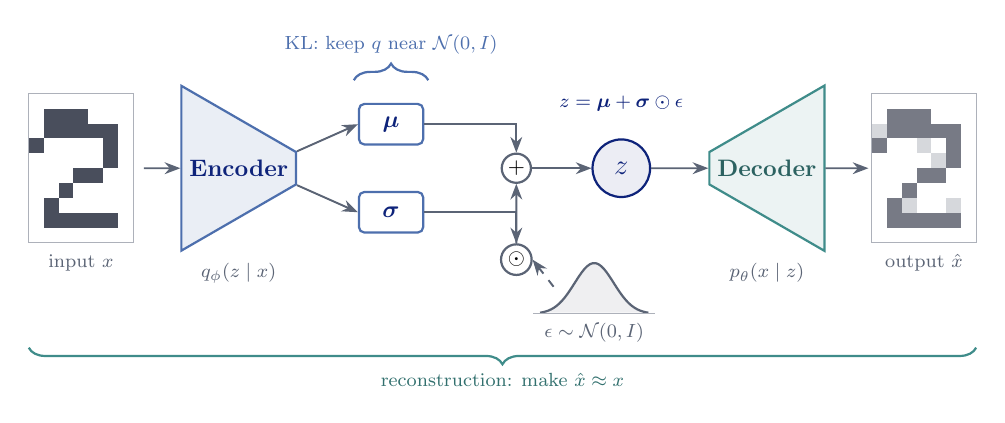
\begin{tikzpicture}[scale=0.86,every node/.append style={transform shape},
    >={Stealth[length=2mm]},
    font=\small,
    arr/.style={->,line width=0.7pt,draw=slate},
    lbl/.style={font=\footnotesize,text=slate,align=center},
    block/.style={trapezium,trapezium stretches=true,minimum width=2.4cm,minimum height=1.55cm,
                  line width=0.8pt,font=\bfseries},
    param/.style={rectangle,rounded corners=2pt,minimum width=0.95cm,minimum height=0.6cm,
                  draw=steel,line width=0.8pt,fill=white,text=navy,font=\normalsize},
    op/.style={circle,draw=slate,line width=0.8pt,fill=white,inner sep=1pt},
  ]

  % ---------- input image x ----------
  \begin{scope}[shift={(0,-0.9)},visible on=<1->]
    \foreach \x/\y in {1/7,2/7,3/7,4/7,5/6,5/5,4/4,3/4,2/3,1/2,1/1,2/1,3/1,4/1,5/1,
                       0/6,2/8,3/8,1/8,5/7}
      \fill[ink!80] (\x*0.22,\y*0.22) rectangle ++(0.22,0.22);
    \draw[slate!50] (0,0) rectangle (1.54,2.2);
    \node[lbl] at (0.77,-0.3) {input $x$};
  \end{scope}

  % ---------- encoder ----------
  \node[block,shape border rotate=270,fill=steel!12,draw=steel,text=navy,
        visible on=<1->,focus on=<1>] (enc) at (3.1,0.2) {Encoder};
  \node[lbl,visible on=<1->] at (3.1,-1.35) {$q_\phi(z\mid x)$};
  \draw[arr,visible on=<1->] (1.7,0.2) -- (enc.west);

  % ---------- mu, sigma ----------
  \node[param,visible on=<2->,focus on=<2>] (mu) at (5.35,0.85) {$\bm{\mu}$};
  \node[param,visible on=<2->,focus on=<2>] (sg) at (5.35,-0.45) {$\bm{\sigma}$};
  \draw[arr,visible on=<2->] (enc.east) ++(0,0.25) -- (mu.west);
  \draw[arr,visible on=<2->] (enc.east) ++(0,-0.25) -- (sg.west);

  % ---------- reparameterisation ----------
  \node[op,visible on=<3->,focus on=<3>] (plus) at (7.2,0.2) {$+$};
  \node[op,inner sep=1.2pt,visible on=<3->,focus on=<3>] (times) at (7.2,-1.15) {$\odot$};
  \draw[arr,visible on=<3->] (mu.east) -| (plus.north);
  \draw[arr,visible on=<3->] (sg.east) -| (times.north);
  \draw[arr,visible on=<3->] (times) -- (plus);

  \begin{scope}[shift={(8.35,-1.95)},visible on=<3->]
    \fill[slate!10] plot[domain=-0.8:0.8,samples=40] (\x,{0.75*exp(-6*\x*\x)}) -- cycle;
    \draw[slate,line width=0.8pt] plot[domain=-0.8:0.8,samples=40] (\x,{0.75*exp(-6*\x*\x)});
    \draw[slate!50] (-0.9,0) -- (0.9,0);
    \node[lbl] at (0,-0.28) {$\epsilon\sim\mathcal{N}(0,I)$};
  \end{scope}
  \draw[arr,dashed,visible on=<3->] (7.75,-1.55) -- (times.east);

  \node[circle,fill=navy!8,draw=navy,line width=0.8pt,text=navy,minimum size=0.85cm,font=\large,
        visible on=<3->,focus on=<3>] (z) at (8.75,0.2) {$z$};
  \draw[arr,visible on=<3->] (plus) -- (z);
  \node[lbl,visible on=<3->,text=navy] at (8.75,1.15) {$z=\bm{\mu}+\bm{\sigma}\odot\epsilon$};

  % ---------- decoder ----------
  \node[block,shape border rotate=90,fill=teal!10,draw=teal,text=teal!70!black,
        visible on=<4->,focus on=<4>] (dec) at (10.9,0.2) {Decoder};
  \node[lbl,visible on=<4->] at (10.9,-1.35) {$p_\theta(x\mid z)$};
  \draw[arr,visible on=<4->] (z) -- (dec.west);

  % ---------- reconstruction x-hat ----------
  \begin{scope}[shift={(12.45,-0.9)},visible on=<4->]
    \foreach \x/\y in {1/7,2/7,3/7,4/7,5/6,5/5,4/4,3/4,2/3,1/2,1/1,2/1,3/1,4/1,5/1,
                       0/6,2/8,3/8,1/8,5/7}
      \fill[ink!60] (\x*0.22,\y*0.22) rectangle ++(0.22,0.22);
    \foreach \x/\y in {0/7,4/5,2/2,5/2,3/6}
      \fill[slate!25] (\x*0.22,\y*0.22) rectangle ++(0.22,0.22);
    \draw[slate!50] (0,0) rectangle (1.54,2.2);
    \node[lbl] at (0.77,-0.3) {output $\hat{x}$};
  \end{scope}
  \draw[arr,visible on=<4->] (dec.east) -- (12.4,0.2);

  % ---------- loss braces ----------
  \draw[visible on=<5->,decorate,decoration={brace,amplitude=6pt,mirror},teal,line width=0.8pt]
       (0,-2.45) -- (13.99,-2.45)
       node[midway,below=7pt,text=teal!80!black,font=\footnotesize] {reconstruction: make $\hat{x}\approx x$};
  \draw[visible on=<5->,decorate,decoration={brace,amplitude=6pt},steel,line width=0.8pt]
       (4.8,1.5) -- (5.9,1.5)
       node[midway,above=7pt,text=steel,font=\footnotesize] {KL: keep $q$ near $\mathcal{N}(0,I)$};
\end{tikzpicture}

\vspace{-4pt}
\only<5>{%
  \begin{beamercolorbox}[rounded=true,wd=0.8\linewidth,center,sep=4pt]{block body}
    \centering\small
    $\mathcal{L}(\theta,\phi;x)=
      \underbrace{\mathbb{E}_{q_\phi(z\mid x)}\!\left[\log p_\theta(x\mid z)\right]}_{\color{teal}\text{reconstruction}}
      \;-\;
      \underbrace{D_{\text{KL}}\!\left(q_\phi(z\mid x)\,\|\,p(z)\right)}_{\color{steel}\text{regularisation}}$
  \end{beamercolorbox}}
\only<1-4>{\vspace{1.25cm}}
\end{frame}

\end{document}
